
\frame{\frametitle{Two different approaches}
  Solve $Ax=b$

  Direct methods:
  \begin{itemize}
  \item Deterministic
  \item Exact up to machine precision
  \item Expensive (in time and space)
  \end{itemize}
  Iterative methods:
  \begin{itemize}
  \item Only approximate
  \item Cheaper in space and (possibly) time
  \item Convergence not guaranteed
  \end{itemize}
}

\frame{\frametitle{Iterative methods}
  Choose any $x_0$ and repeat
  \[ x^{k+1}=Bx^k+c \]
  until $\|x^{k+1}-x^k\|_2<\epsilon$
  or until $\frac{\|x^{k+1}-x^k\|_2}{\|x^k\|}<\epsilon$
}

\frame{\frametitle{Example of iterative solution}

 Example system
\[ \left(\begin{matrix}10&0&1\\ 1/2&7&1\\ 1&0&6\end{matrix}\right)
  \left(
    \begin{matrix}
      x_1\\ x_2\\ x_3
    \end{matrix}\right) = 
    \left(\begin{matrix}
      21\\ 9\\ 8
    \end{matrix}\right)
\]
with solution $(2,1,1)$.

 Suppose you know (physics) that solution components are roughly
  the same size, and observe the dominant size of the diagonal, then
\[ \left(\begin{matrix}10&\\ &7\\ &&6\end{matrix}\right)
  \left(
    \begin{matrix}
      x_1\\ x_2\\ x_3
    \end{matrix}\right) = 
    \left(\begin{matrix}
      21\\ 9\\ 8
    \end{matrix}\right)
\]
might be a good approximation: solution $(2.1,9/7,8/6)$.
}

\frame{\frametitle{Iterative example$'$}
 Example system
\[ \left(\begin{matrix}10&0&1\\ 1/2&7&1\\ 1&0&6\end{matrix}\right)
  \left(
    \begin{matrix}
      x_1\\ x_2\\ x_3
    \end{matrix}\right) = 
    \left(\begin{matrix}
      21\\ 9\\ 8
    \end{matrix}\right)
\]
with solution $(2,1,1)$.

 Also easy to solve:
\[ \left(\begin{matrix}10\\ 1/2&7\\ 1&0&6\end{matrix}\right)
  \left(
    \begin{matrix}
      x_1\\ x_2\\ x_3
    \end{matrix}\right) = 
    \left(\begin{matrix}
      21\\ 9\\ 8
    \end{matrix}\right)
\]
with solution $(2.1,7.95/7,5.9/6)$.
}

\frame{\frametitle{Abstract presentation}

\begin{itemize}
\item To solve $Ax=b$; too expensive; suppose $K\approx A$ and solving
  $Kx=b$ is possible
\item Define $Kx_0=b$, then error correction $x_0=x+e_0$, and
  $A(x_0-e_0)=b$
\item so $Ae_0=Ax_0-b=r_0$; this is again unsolvable, so
\item $K\tilde e_0$ and $x_1=x_0-\tilde e_0$.
\item now iterate: $e_1=x_1-x$, $Ae_1=Ax_1-b=r_1$ et cetera
\end{itemize}
}

\frame{\frametitle{Error analysis}

\begin{itemize}
\item One step
\begin{eqnarray}
r_1&=&Ax_1-b=A(x_0-\tilde e_0)-b\\
&=&r_0-AK\inv r_0\\
&=&(I-AK\inv)r_0
\end{eqnarray}
\item Inductively: $r_n=(I-AK\inv)^nr_0$ so $r_n\downarrow0$ if
  $|\lambda(I-AK\inv)|<1$\\ Geometric reduction (or amplification!)
\item This is `stationary iteration': every iteration step the
  same. Simple analysis, limited applicability.
\end{itemize}
}

\frame[containsverbatim]{\frametitle{Choice of $K$}
  \begin{itemize}
  \item The closer $K$ is to $A$, the faster convergence.
  \item Diagonal and lower triangular choice mentioned above: let \[
    A=D_A+L_A+U_A \] be a splitting into diagonal, lower triangular,
    upper triangular part, then
  \item Jacobi method: $K=D_A$ (diagonal part),
  \item Gauss-Seidel method: $K=D_A+L_A$ (lower triangle, including diagonal)
  \item SOR method: $K=\omega D_A+L_A$
  \end{itemize}
}

\frame[containsverbatim]{\frametitle{Choice of $K$ through incomplete LU}
  \begin{itemize}
  \item Inspiration from direct methods: let $K=LU\approx A$
  \end{itemize}
Gauss elimination:
\begin{verbatim}
for k,i,j:
   a[i,j] = a[i,j] - a[i,k] * a[k,j] / a[k,k]
\end{verbatim}
Incomplete variant:
\begin{verbatim}
for k,i,j:
  if a[i,j] not zero:
    a[i,j] = a[i,j] - a[i,k] * a[k,j] / a[k,k]
\end{verbatim}
$\Rightarrow$ sparsity of $L+U$ the same as of $A$
}

\frame{\frametitle{General form of iterative methods}

Iterative scheme:
\[   x_{i+1} = x_0+K\inv \pi^{(i)}(AK\inv) r_0 \]
Multiply by~$A$ and subtract~$b$:
\[ r_{i+1} = r_0+\tilde\pi^{(i)}(AK\inv)r_0 \]
So:
\[ r_i = \hat\pi^{(i)}(AK\inv) r_0 \]
where $\hat\pi^{(i)}$ is a polynomial of degree~$i$ with
$\hat\pi^{(i)}(0)=\nobreak1$. 

$\Rightarrow$ convergence theory
}

\frame{\frametitle{General form of iterative methods 2.}
\[
  r_{i+1}\gamma_{i+1,i}=AK\inv r_i+\sum_{j\leq i} r_j\gamma_{ji}
\]
and $\gamma_{i+1,i}=\sum_{j\leq i}\gamma_{ji}$.

Write this as $AK\inv R=RH$ where
\[ H=
\begin{pmatrix}
  -\gamma_{11}&-\gamma_{12}&\ldots\\
  \gamma_{21}&-\gamma_{22}&-\gamma_{23}&\ldots\\
  0&\gamma_{32}&-\gamma_{33}&-\gamma_{34}\\
  \emptyset&\ddots&\ddots&\ddots&\ddots
\end{pmatrix}
\]
$H$ is a Hessenberg matrix, and note zero column sums.

Divide $A$ out:
\[
  x_{i+1}\gamma_{i+1,i}=K\inv r_i+\sum_{j\leq i} x_j\gamma_{ji}
\]
}

\frame{\frametitle{Orthogonality}
Idea one:
\begin{quote}
  If you can make all your residuals orthogonal to each other, and the
  matrix is of dimension~$n$, then after $n$ iterations you have to
  have converged: it is not possible to have an $n+1$-st residuals
  that is orthogonal and nonzero.
\end{quote}
Idea two:
\begin{quote}
  The sequence of residuals spans a series of subspaces of increasing
  dimension, and by orthogonalizing the initial residual is projected on
  these spaces. This means that the errors will have decreasing sizes.
\end{quote}
}

\frame{
  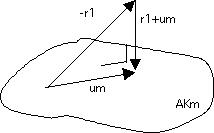
\includegraphics[scale=.7]{graphics/projection}
}

\frame{\frametitle{Full Orthogonalization Method}

\begin{quote}
  \begin{tabbing}
    Let $r_0$ be given\\
    For \=$i\geq 0$:\\
    \>let $s\leftarrow K\inv r_i$\\
    \>let $t\leftarrow AK\inv r_i$\\
    \>for \=$j\leq i$:\\
    \>\>let $\gamma_j$ be the coefficient so that $t-\gamma_jr_j\perp r_j$\\
    \>for \=$j\leq i$:\\
    \>\>form \=$s\leftarrow s-\gamma_jx_j$\\
    \>\>and  \>$t\leftarrow t-\gamma_jr_j$\\
    \>let $x_{i+1}=(\sum_j\gamma_j)\inv s$,
    $r_{i+1}=(\sum_j\gamma_j)\inv t$.\\
  \end{tabbing}
\end{quote}
}

\frame{\frametitle{Conjugate Gradients}
Basic idea:
\[ r_i^tK\inv r_j=0\quad\hbox{if $i\not=j$}. \]
Split recurrences:
\[
  \begin{cases}
    x_{i+1}=x_i-\delta_i p_i \\
    r_{i+1}=r_i-\delta_iA p_i \\
    p_i = K\inv r_i+\sum_{j<i}\gamma_{ij} p_j,
  \end{cases}
\]
}

\frame{\frametitle{Symmetric Positive Definite case}
  Three term recurrence is enough:
\[
  \begin{cases}
    x_{i+1}=x_i-\delta_i p_i \\
    r_{i+1}=r_i-\delta_iA p_i \\
    p_{i+1} = K\inv r_{i+1}+\gamma_i p_i
  \end{cases}
\]
}

\frame{\frametitle{Preconditioned Conjugate Gradietns}
\small
\input pcg
}

\frame{\frametitle{Observations on iterative methods}
  \begin{itemize}
  \item Conjugate gradients: constant storage and inner products;
    works only for symmetric systems
    \item GMRES (like FOM): growing storage and inner products:
      restarting and numerical cleverness
    \item BiCGstab and QMR: relax the orthogonality
  \end{itemize}
}

\frame{\frametitle{CG derived from minimization}
Special case of SPD:
\begin{equation}
  \hbox{For which vector $x$ with $\|x\|=1$ is $f(x)=1/2 x^tAx-b^tx$ minimal?}
\end{equation}
Taking derivative:
\[ f'(x) = Ax-b. \]
Update
\[ x_{i+1} = x_i+p_i\delta_i \]
optimal value:
\[ \delta_i = \argmin_\delta \| f(x_i+p_i\delta) \| 
=\frac{r_i^tp_i}{p_1^tAp_i} 
\]
Other constants follow from orthogonality.
}
